\documentclass[a4paper,12pt]{report}

\usepackage[utf8]{inputenc}
\usepackage[T1]{fontenc}
\usepackage[english]{babel}
\usepackage{graphicx}
\usepackage{hyperref}
\usepackage{listings}
\usepackage{xcolor}
\usepackage{float}
\usepackage{booktabs}
\usepackage{tikz}
\usetikzlibrary{shapes,arrows,positioning,fit,calc}
\usepackage{caption}
\usepackage{geometry}
\geometry{margin=2.5cm}

\definecolor{codegreen}{rgb}{0,0.6,0}
\definecolor{codegray}{rgb}{0.5,0.5,0.5}
\definecolor{codepurple}{rgb}{0.58,0,0.82}
\definecolor{backcolour}{rgb}{0.95,0.95,0.92}

\lstdefinestyle{mystyle}{
    backgroundcolor=\color{backcolour},
    commentstyle=\color{codegreen},
    keywordstyle=\color{magenta},
    numberstyle=\tiny\color{codegray},
    stringstyle=\color{codepurple},
    basicstyle=\ttfamily\footnotesize,
    breakatwhitespace=false,
    breaklines=true,
    captionpos=b,
    keepspaces=true,
    numbers=left,
    numbersep=5pt,
    showspaces=false,
    showstringspaces=false,
    showtabs=false,
    tabsize=2
}

\lstset{style=mystyle}

\newcommand{\placeholder}[2][\textwidth]{%
  \begin{center}
  \fbox{%
    \begin{minipage}{#1}
      \centering\vspace{1cm}
      {\Large \textbf{#2}}\\[0.3cm]
      {\footnotesize \textit{Immagine da inserire}}\vspace{1cm}
    \end{minipage}%
  }
  \end{center}
}

\title{
    \vspace{3cm}
    \Huge\textbf{Smart Home IoT System}\\[0.5cm]
    \Large{Software Engineering for the Internet of Things}\\[0.3cm]
    \large{Project Report}
}

\author{
    Alessandro Di Giacomo\\[0.3cm]
    Graziano D'Agostino\\[0.3cm]
    Agostino D'Agostino\\[0.3cm]
    \textit{Università degli Studi dell'Aquila}
}

\date{\today}

\begin{document}

\maketitle

\tableofcontents
\newpage

% ===========================================================================
\chapter*{Objective}
\addcontentsline{toc}{chapter}{Objective}
% ===========================================================================

The project requires a complete IoT system that collects, processes, stores,
and visualises data from different domains. The system should show key IoT
concepts and work across multiple application areas. We built a Smart Home
implementation that goes from sensor data acquisition to visualisation and
automated actuation, with all components containerised for portable deployment.

The six points of the project scope are addressed as follows. Sensors are
simulated in software for data collection. Node-RED is the middleware
processing layer. InfluxDB provides time-series storage. Grafana renders an
interactive dashboard. Configurable thresholds drive Telegram-based alerting.
Every component runs as a Docker container orchestrated through Docker
Compose.

\begin{figure}[H]
\centering
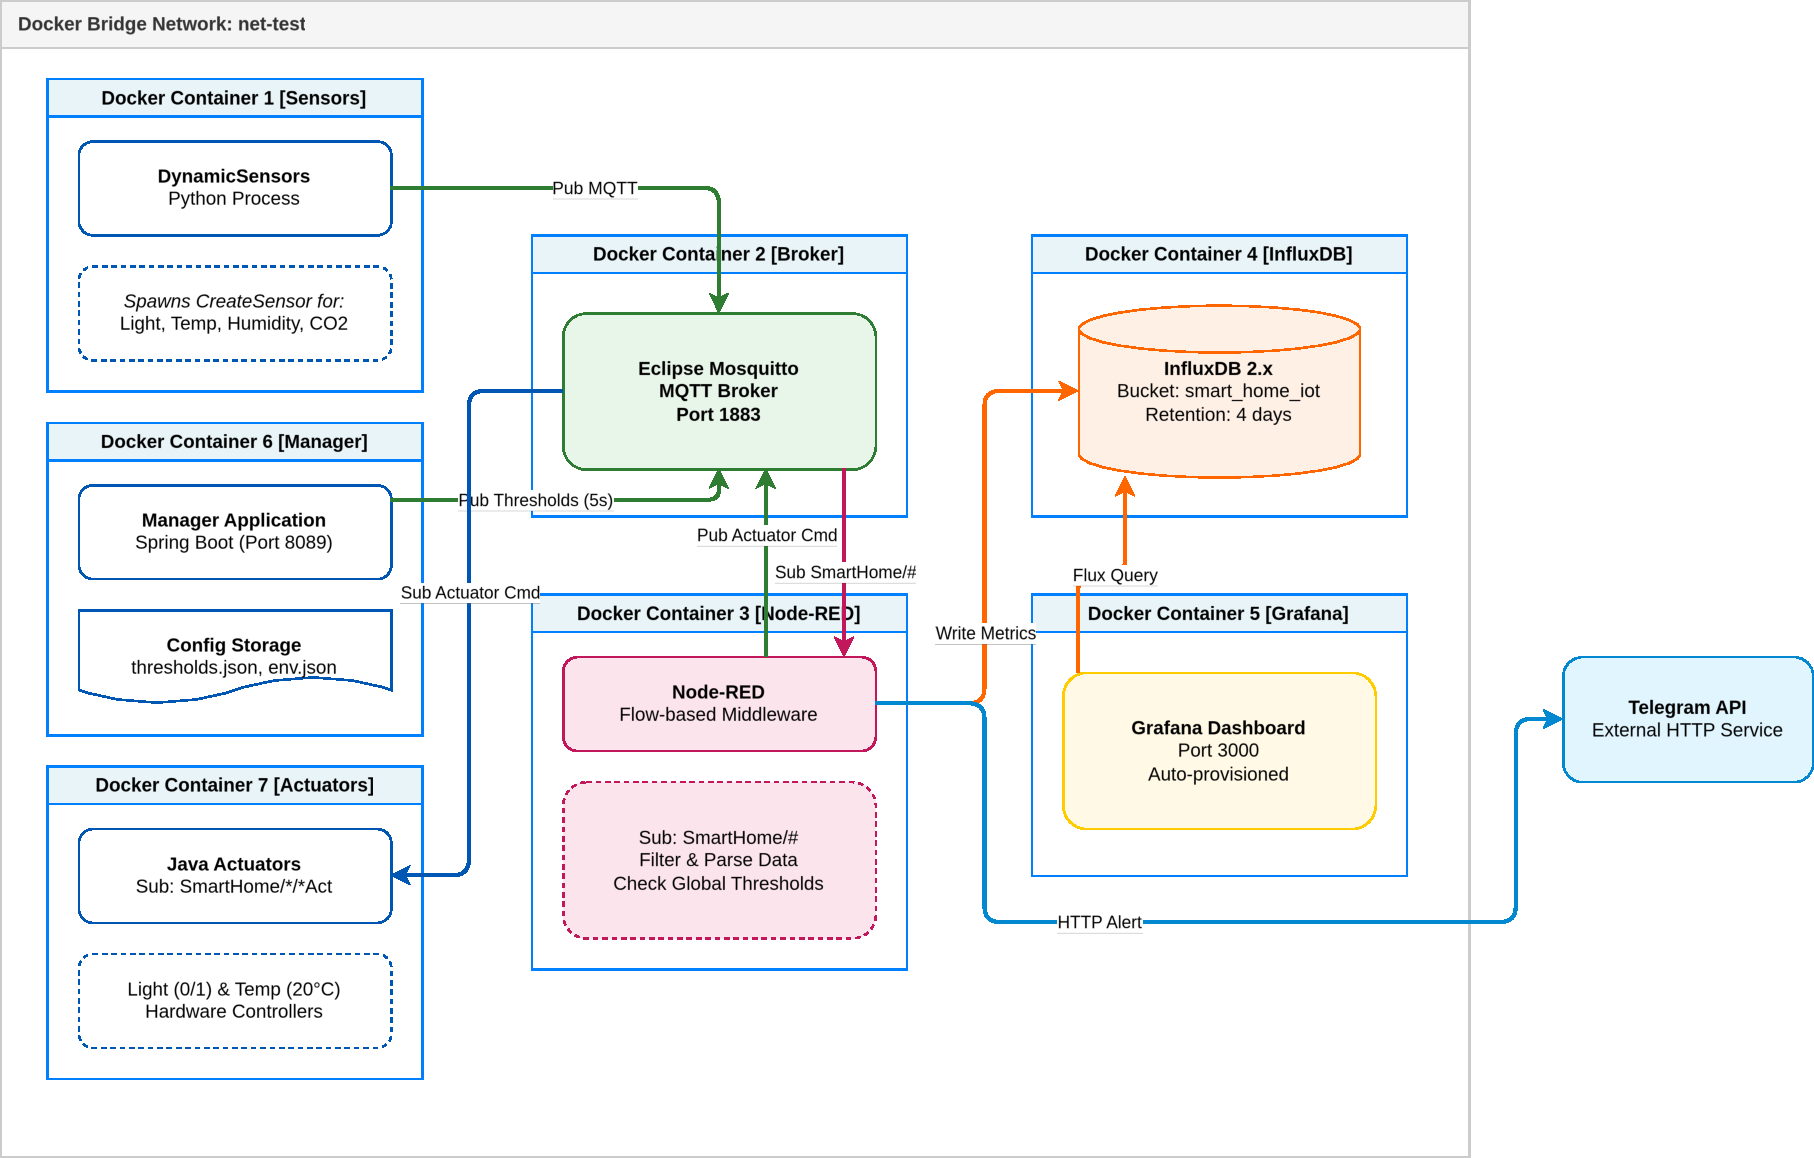
\includegraphics[width=0.9\textwidth]{images/architecture-diagram.pdf}
\caption{System architecture: MQTT communication between sensors, broker,
         and applications in a containerised environment.}
\label{fig:architecture}
\end{figure}

\vfill

% ===========================================================================
\chapter*{Architecture Overview}
\addcontentsline{toc}{chapter}{Architecture Overview}
% ===========================================================================

The system architecture is organised in two complementary views, as shown
in Figure~\ref{fig:ref-architecture}. The upper part illustrates the
Docker-based deployment: seven containers (Sensors, Broker, Node-RED,
InfluxDB, Grafana, Manager, Actuators) communicate over a shared bridge
network via MQTT, HTTP, and InfluxDB protocols. The lower part abstracts
the same system into four logical layers Device \& Data,
Communication, Middleware \& Storage, and Application highlighting how
data flows from physical sensors through the MQTT broker and processing
pipeline up to the visualisation and management dashboards.

\begin{figure}[H]
\centering
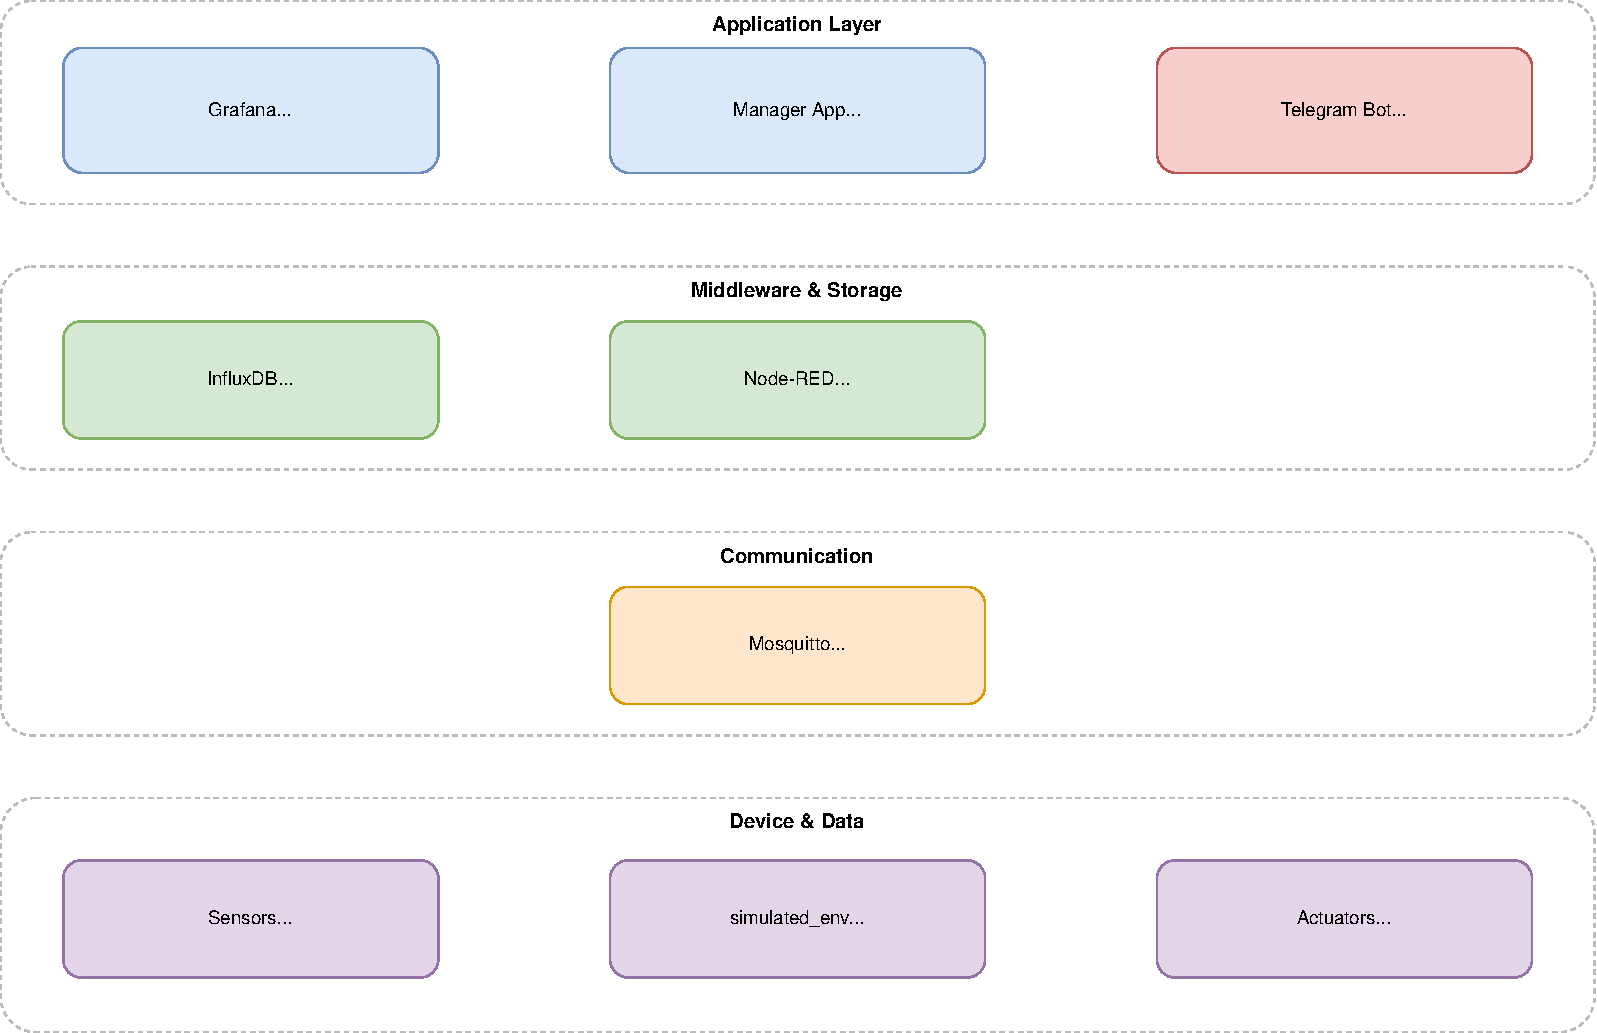
\includegraphics[width=0.8\textwidth]{images/architecture-reference.pdf}
\caption{System architecture: Docker deployment view (top) and logical
         layered view (bottom).}
\label{fig:ref-architecture}
\end{figure}

This layered structure means each component can evolve independently. Adding
a new sensor type does not require changes to Node-RED or Grafana, and
replacing the visualisation tool would not affect data collection.

\begin{figure}[H]
\centering
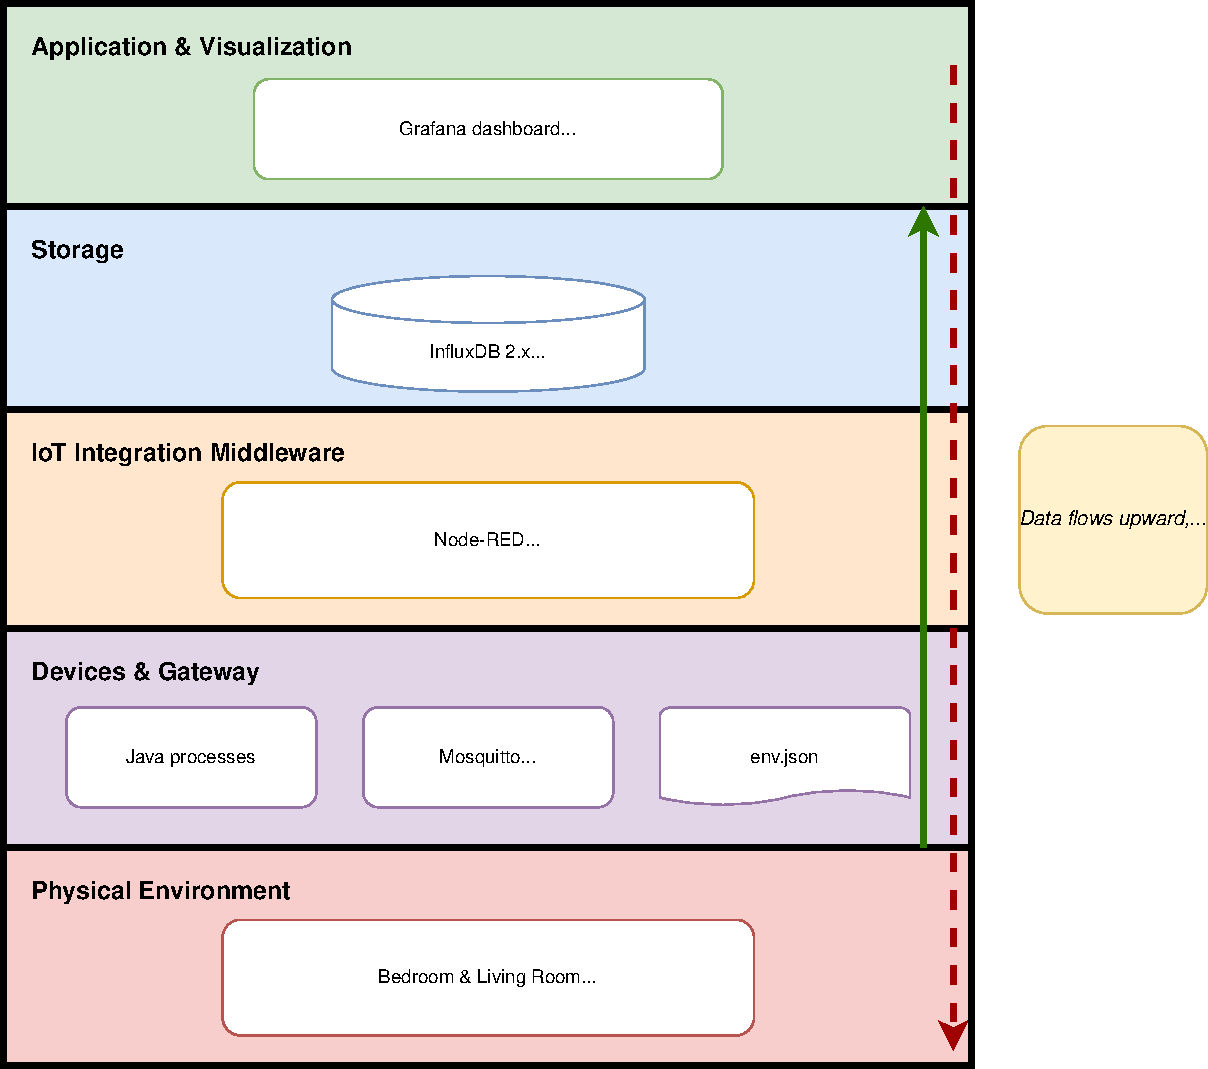
\includegraphics[width=0.8\textwidth]{images/block-architecture.pdf}
\caption{Layered block architecture diagram.}
\label{fig:block-architecture}
\end{figure}

% ===========================================================================
\chapter*{Applicable Domains}
\addcontentsline{toc}{chapter}{Applicable Domains}
% ===========================================================================

The requirement document lists six possible application domains: Smart
Agriculture, Smart Cities, Industrial IoT, Environmental Monitoring,
Healthcare, and Smart Homes. We chose the \textbf{Smart Home} domain. Two
rooms (bedroom and living room) are monitored for light intensity,
temperature, humidity, and CO\textsubscript{2} concentration. Actuators for
lighting and temperature set-points provide automatic responses to threshold
violations.

We picked Smart Home because it is familiar and involves multiple sensor
types: scalar measurements (temperature, light), percentage-based
readings (humidity), and binary or set-point actuation (light on/off,
temperature target).

% ===========================================================================
\chapter*{Functional Requirements}
\addcontentsline{toc}{chapter}{Functional Requirements}
% ===========================================================================

% ---------------------------------------------------------------------------
\section*{1. Sensor Integration}
\addcontentsline{toc}{section}{1. Sensor Integration}
% ---------------------------------------------------------------------------

The requirements ask for simulated or real sensors that publish data
periodically with realistic ranges, timestamps, and unique identifiers.

We built the sensor subsystem in Java 17 with two classes.
\texttt{DynamicSensors.java} is the entry point. It polls the shared
environment file \texttt{simulated\_env/env.json} every five seconds and
starts a \texttt{CreateSensor} process for each sensor entry it
finds. Sensors can be added or removed at runtime without restarting
anything.

\begin{figure}[H]
\centering
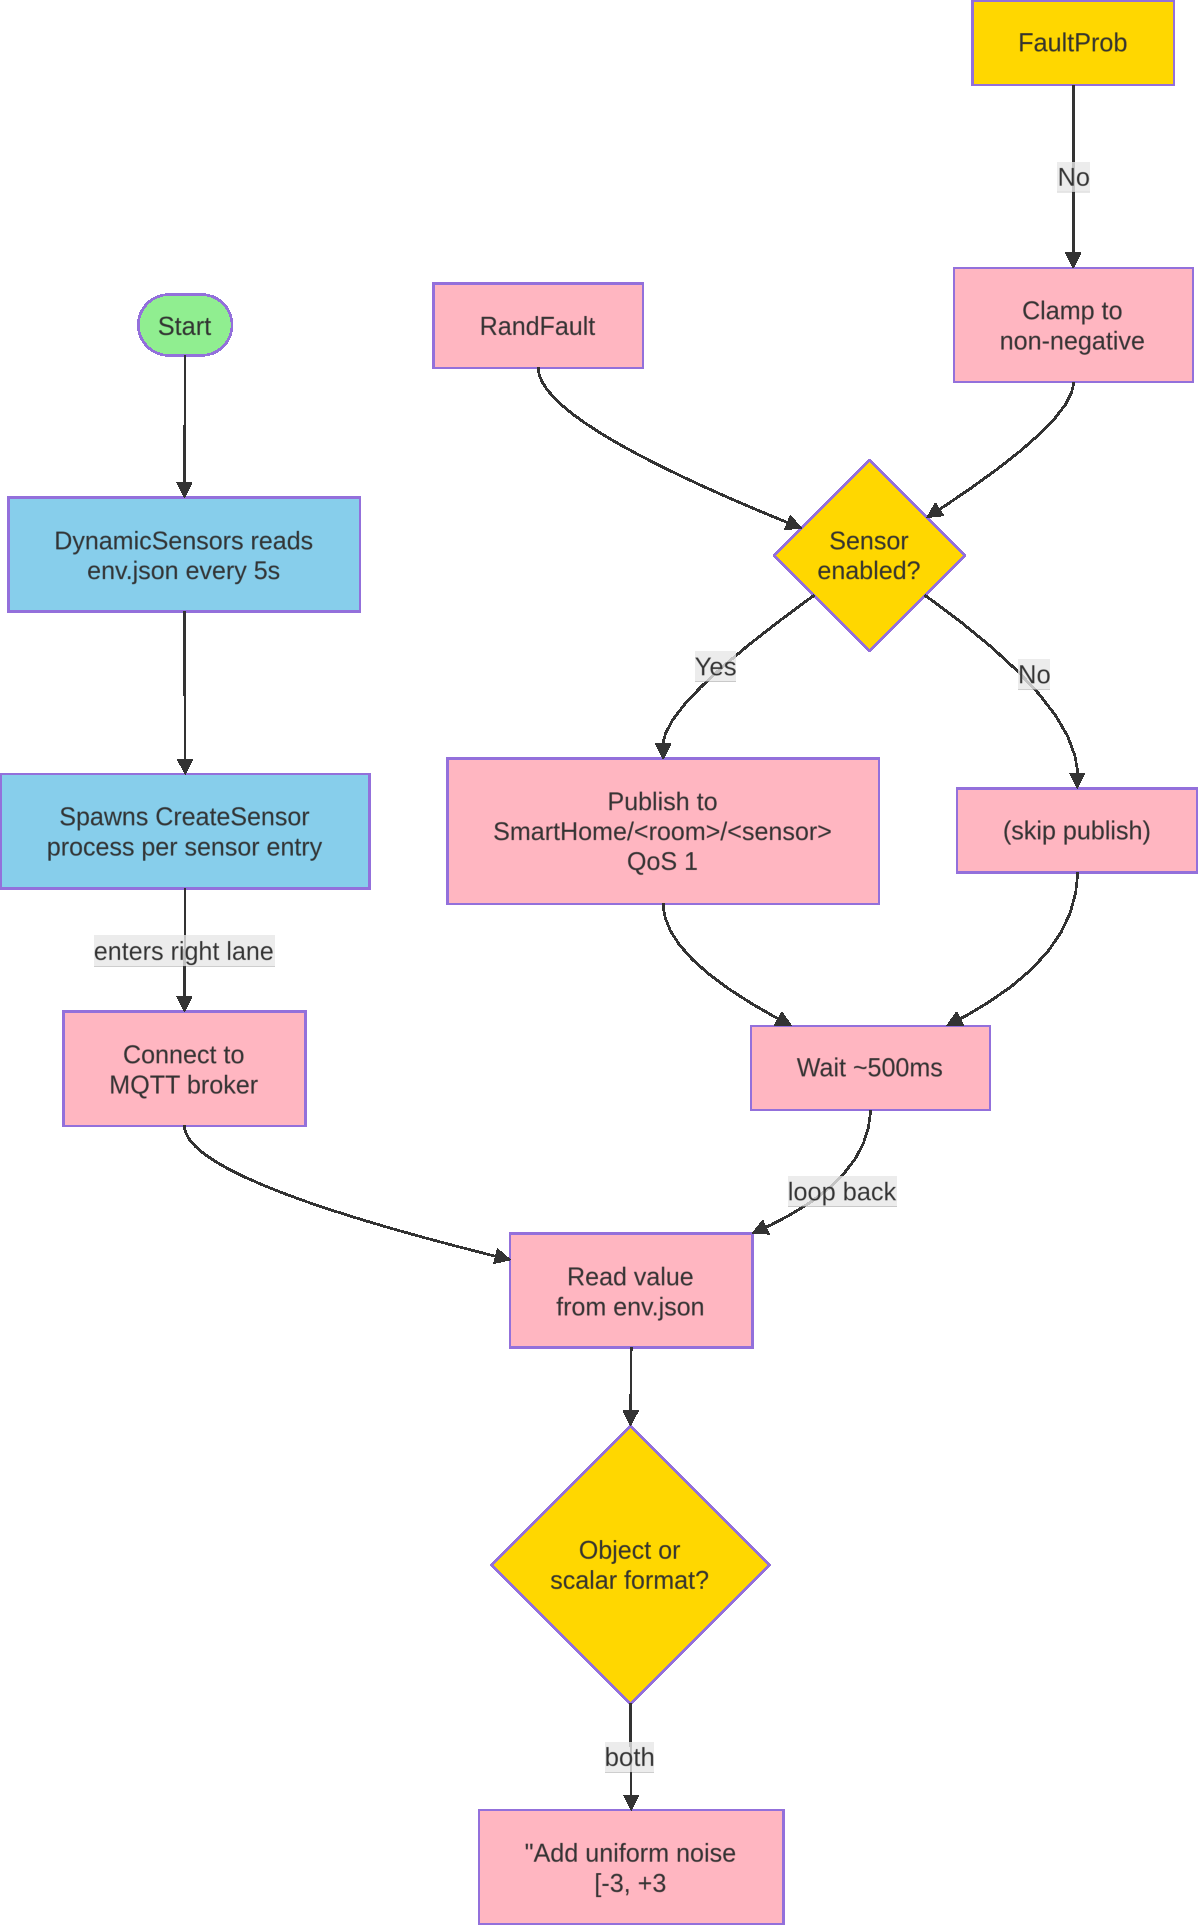
\includegraphics[width=0.8\textwidth]{images/sensor-cycle.pdf}
\caption{Sensor operation cycle.}
\label{fig:sensor-cycle}
\end{figure}

Each \texttt{CreateSensor} instance connects to the MQTT broker and enters a
publishing loop. On each iteration it reads the sensor value from
\texttt{env.json}. The code handles both scalar values (e.g.,
\texttt{"light": 0}) and structured objects with an \texttt{enabled} flag
(e.g., \texttt{"humidity": \{"value": 30, "enabled": true\}}). It adds uniform
noise drawn from \(\{-3,-2,-1,0,1,2,3\}\) to the base value and clamps the
result to non-negative values. With 1\% probability the value is replaced with
a random integer between 6 and 10 to simulate faults. The result is published
as a string to \texttt{SmartHome/<room>/<sensor>} with QoS 1, roughly every
500 milliseconds. If a sensor is disabled, the process skips publishing.

Four sensor types are deployed across the two rooms: light, temperature,
humidity, and CO\textsubscript{2}. Each topic combines the room name and
sensor type, so every data stream has a unique identifier.

% ---------------------------------------------------------------------------
\section*{2. Communication Protocols}
\addcontentsline{toc}{section}{2. Communication Protocols}
% ---------------------------------------------------------------------------

The requirements specify MQTT as the primary protocol, with well-structured
topics, a broker, and support for dynamic configuration.

\textbf{Why MQTT.} The course compares several IoT protocols: MQTT, CoAP,
HTTP, AMQP, and DDS. We chose MQTT because it fits the project's needs better
than the alternatives. CoAP uses a request-response model over UDP and is
designed for extremely constrained devices, but our sensors run on Java with
full network stacks where CoAP's lightweight advantages are less relevant.
HTTP, while ubiquitous, follows a pull model that requires polling and
generates significantly more bytes on the wire a drawback for frequent
sensor updates. MQTT's publish-subscribe pattern matches the event-driven
nature of sensor data: readings arrive asynchronously and must be pushed to
multiple consumers (storage, alerting, actuation) without requiring each
consumer to poll. The oneM2M standard, discussed during the course, defines
MQTT as a recognised protocol binding for IoT communication, further
motivating its adoption.

\textbf{QoS choices.} MQTT provides three Quality of Service levels. Sensors
publish with QoS 1 (at least once) to ensure readings are not lost in transit
due to network interruptions, at the cost of possible duplicates. Node-RED
subscribes with QoS 2 (exactly once) for the threshold and alerting path,
where duplicate messages could cause false alarms. The broker (Eclipse
Mosquitto) handles the retry logic automatically, storing undelivered messages
for disconnected subscribers.

\textbf{MQTT broker.} Eclipse Mosquitto runs in its own Docker container on
port 1883. In this development setup the broker allows anonymous connections.
Authentication and TLS would be needed for production.

\begin{sloppypar}
\textbf{Topic hierarchy.} We adapted the suggested pattern
\texttt{/<domain>/<location>/<sensor>} to the Smart Home domain:
\end{sloppypar}

\begin{figure}[H]
\centering
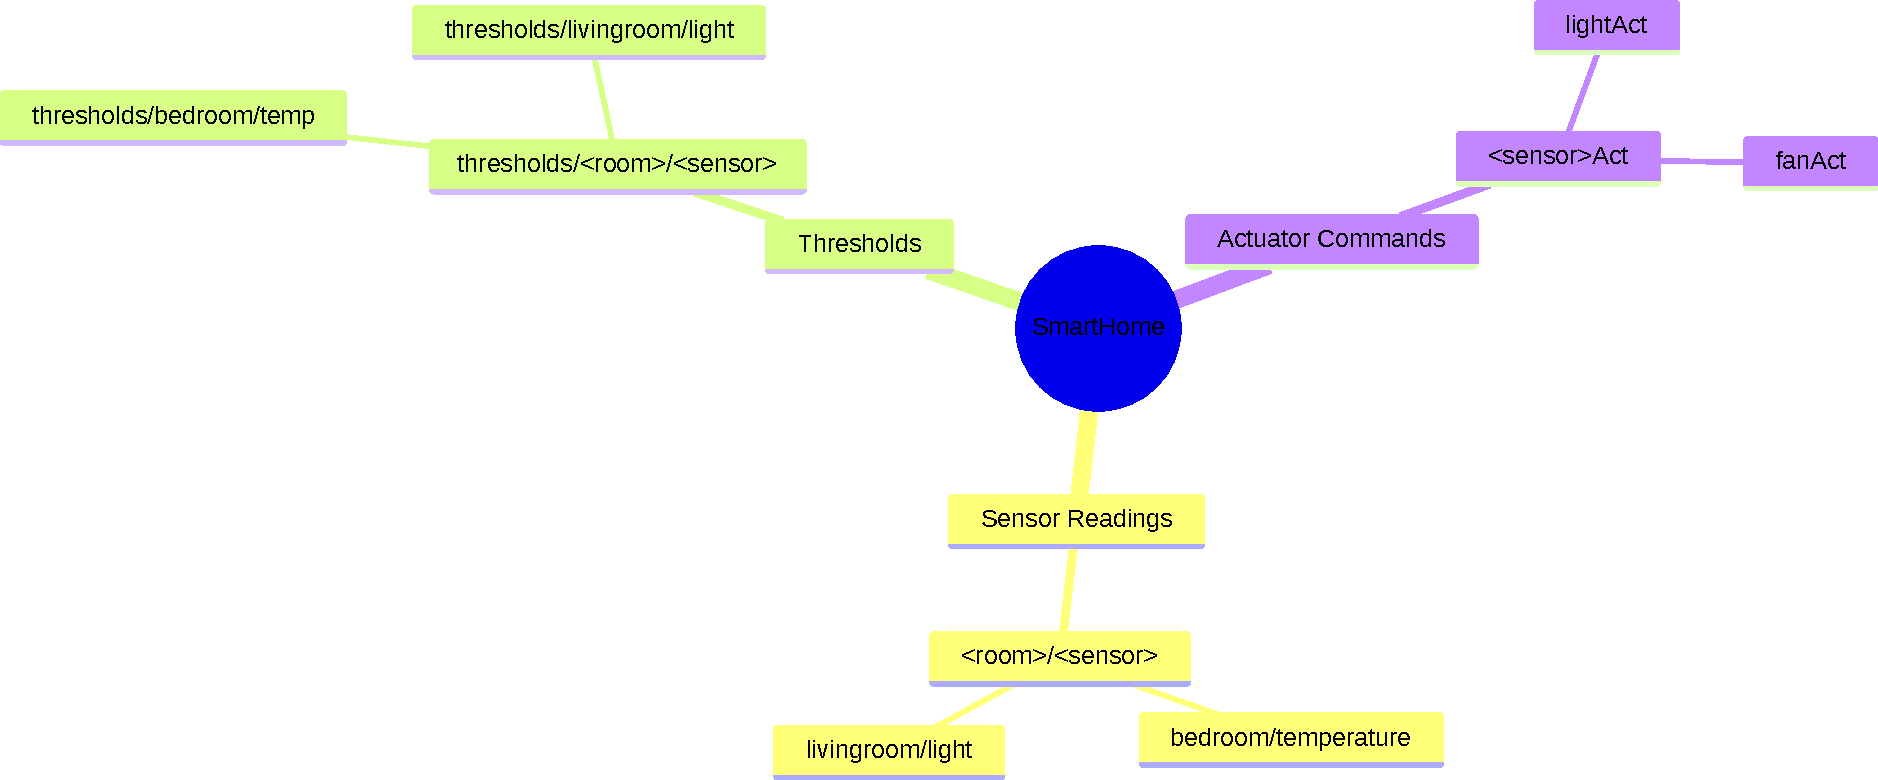
\includegraphics[width=0.8\textwidth]{images/mqtt-topics.pdf}
\caption{MQTT topic hierarchy.}
\label{fig:mqtt-topics}
\end{figure}

\begin{lstlisting}[caption=Struttura dei topic MQTT]
SmartHome/<room>/<sensor>                  # sensor readings
SmartHome/thresholds/<room>/<sensor>       # threshold updates
SmartHome/<room>/<sensor>Act               # actuator commands
\end{lstlisting}

Concrete examples are:
\begin{itemize}
  \item \texttt{SmartHome/bedroom/temperature}
  \item \texttt{SmartHome/thresholds/livingroom/light}
  \item \texttt{SmartHome/bedroom/lightAct}
\end{itemize}
This three-family structure separates
sensor data, configuration, and commands into independent streams.
Subscribers use MQTT wildcards to pick the category they need. Node-RED
subscribes to \texttt{SmartHome/\#} for everything, while an individual
actuator subscribes only to its specific \texttt{Act} topic.

\textbf{Dynamic configuration.} The Manager Application publishes threshold
updates to \texttt{SmartHome/thresholds/<room>/<sensor>} every five seconds.
Node-RED picks up these messages and updates its in-memory thresholds on the
fly. No restart needed when thresholds change.

% ---------------------------------------------------------------------------
\section*{3. Data Processing}
\addcontentsline{toc}{section}{3. Data Processing}
% ---------------------------------------------------------------------------

The requirements ask for a middleware layer that aggregates, transforms, and
enriches sensor data before sending it to storage and visualisation. Node-RED
handles this with its flow-based programming model.

\textbf{Batch vs stream processing.} The course distinguishes two processing
paradigms. Batch processing operates on stored data in fixed time intervals
and is suited for offline analytics. Stream processing, on the other hand,
handles each data point as it arrives, making it appropriate for real-time
monitoring and alerting. Our system is a stream processing architecture: every
MQTT message is processed immediately upon arrival, and the pipeline produces
alerts, database writes, and actuator commands within milliseconds of a sensor
reading. There is no polling or periodic batch job in the critical path. This
approach follows the general data pipeline workflow described in the course
(Data Generation $\rightarrow$ Transformation $\rightarrow$ Ingestion
$\rightarrow$ DB $\rightarrow$ Processing), with the difference that
transformation and processing happen concurrently in Node-RED rather than in
separate stages.

\begin{figure}[H]
\centering
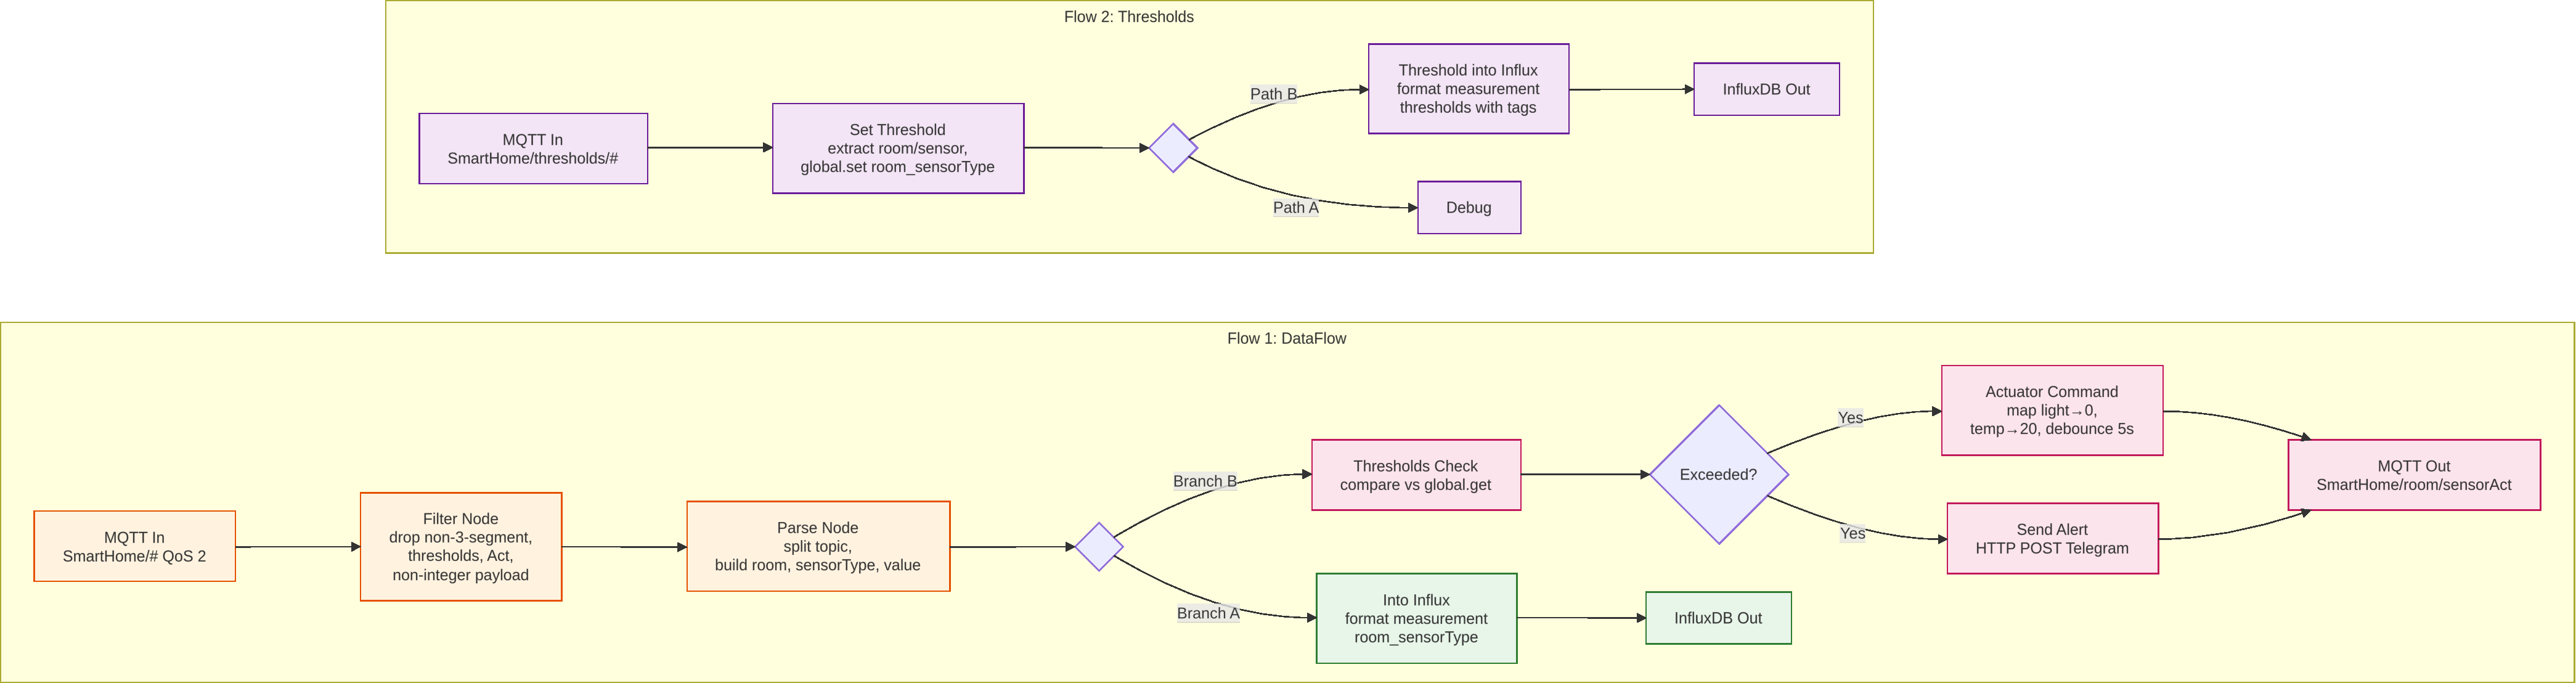
\includegraphics[width=0.8\textwidth]{images/nodered-pipeline.pdf}
\caption{Node-RED processing pipeline.}
\label{fig:nodered-pipeline}
\end{figure}

The processing pipeline has two flows.

\textbf{DataFlow tab.} The main pipeline starts with an MQTT input node
subscribed to \texttt{SmartHome/\#} with QoS 2. A filter node drops any
message whose topic does not have exactly three segments, contains
\texttt{thresholds}, ends in \texttt{Act}, or has a non-integer payload. This
keeps only clean sensor readings. A parsing node splits the topic on
\texttt{/} and builds a structured message with \texttt{room},
\texttt{sensorType}, and \texttt{value}.

From here the flow forks into parallel branches. One branch writes the
measurement to InfluxDB under \texttt{\{room\}\_\{sensorType\}} with tags
\texttt{room} and \texttt{sensorType}. Another branch compares the value
against the threshold from Node-RED's global context using the key
\texttt{\{room\}\_\{sensorType\}}. If the threshold is exceeded, the message
goes to the alerting and actuation sub-flows.

\textbf{Thresholds tab.} A second flow subscribes to
\texttt{SmartHome/thresholds/\#}, extracts room and sensor type from the
topic, updates the corresponding entry in Node-RED's global context, and
writes the change to InfluxDB for auditing.

% ---------------------------------------------------------------------------
\section*{4. Data Storage}
\addcontentsline{toc}{section}{4. Data Storage}
% ---------------------------------------------------------------------------

The requirements specify a time-series database with data tagged by
timestamp, sensor type, location, and domain.

\textbf{Why a time-series database.} Sensor data has specific
characteristics that make relational databases a poor fit. Readings are
immutable and append-only, queries scan contiguous time ranges rather than
random rows, and the write volume is high (multiple sensors publishing every
500 ms). A relational database like PostgreSQL can store this data, but the
schema needs constant updates when sensors are added, write performance
degrades as the table grows, and horizontal scaling is complex. Time-series
databases are built for these workloads: they use columnar compression,
partition data by time for efficient range scans, and support retention
policies that expire old data automatically. The course presents InfluxDB,
Prometheus, and TimescaleDB as options; we chose InfluxDB 2.x for its
integrated query language (Flux), its easy Docker setup, and its compatibility
with Grafana.

We used \textbf{InfluxDB 2.x} with a single bucket called
\texttt{smart\_home\_iot} under organisation \texttt{univaq}. The retention
period is four days.

\begin{figure}[H]
\centering
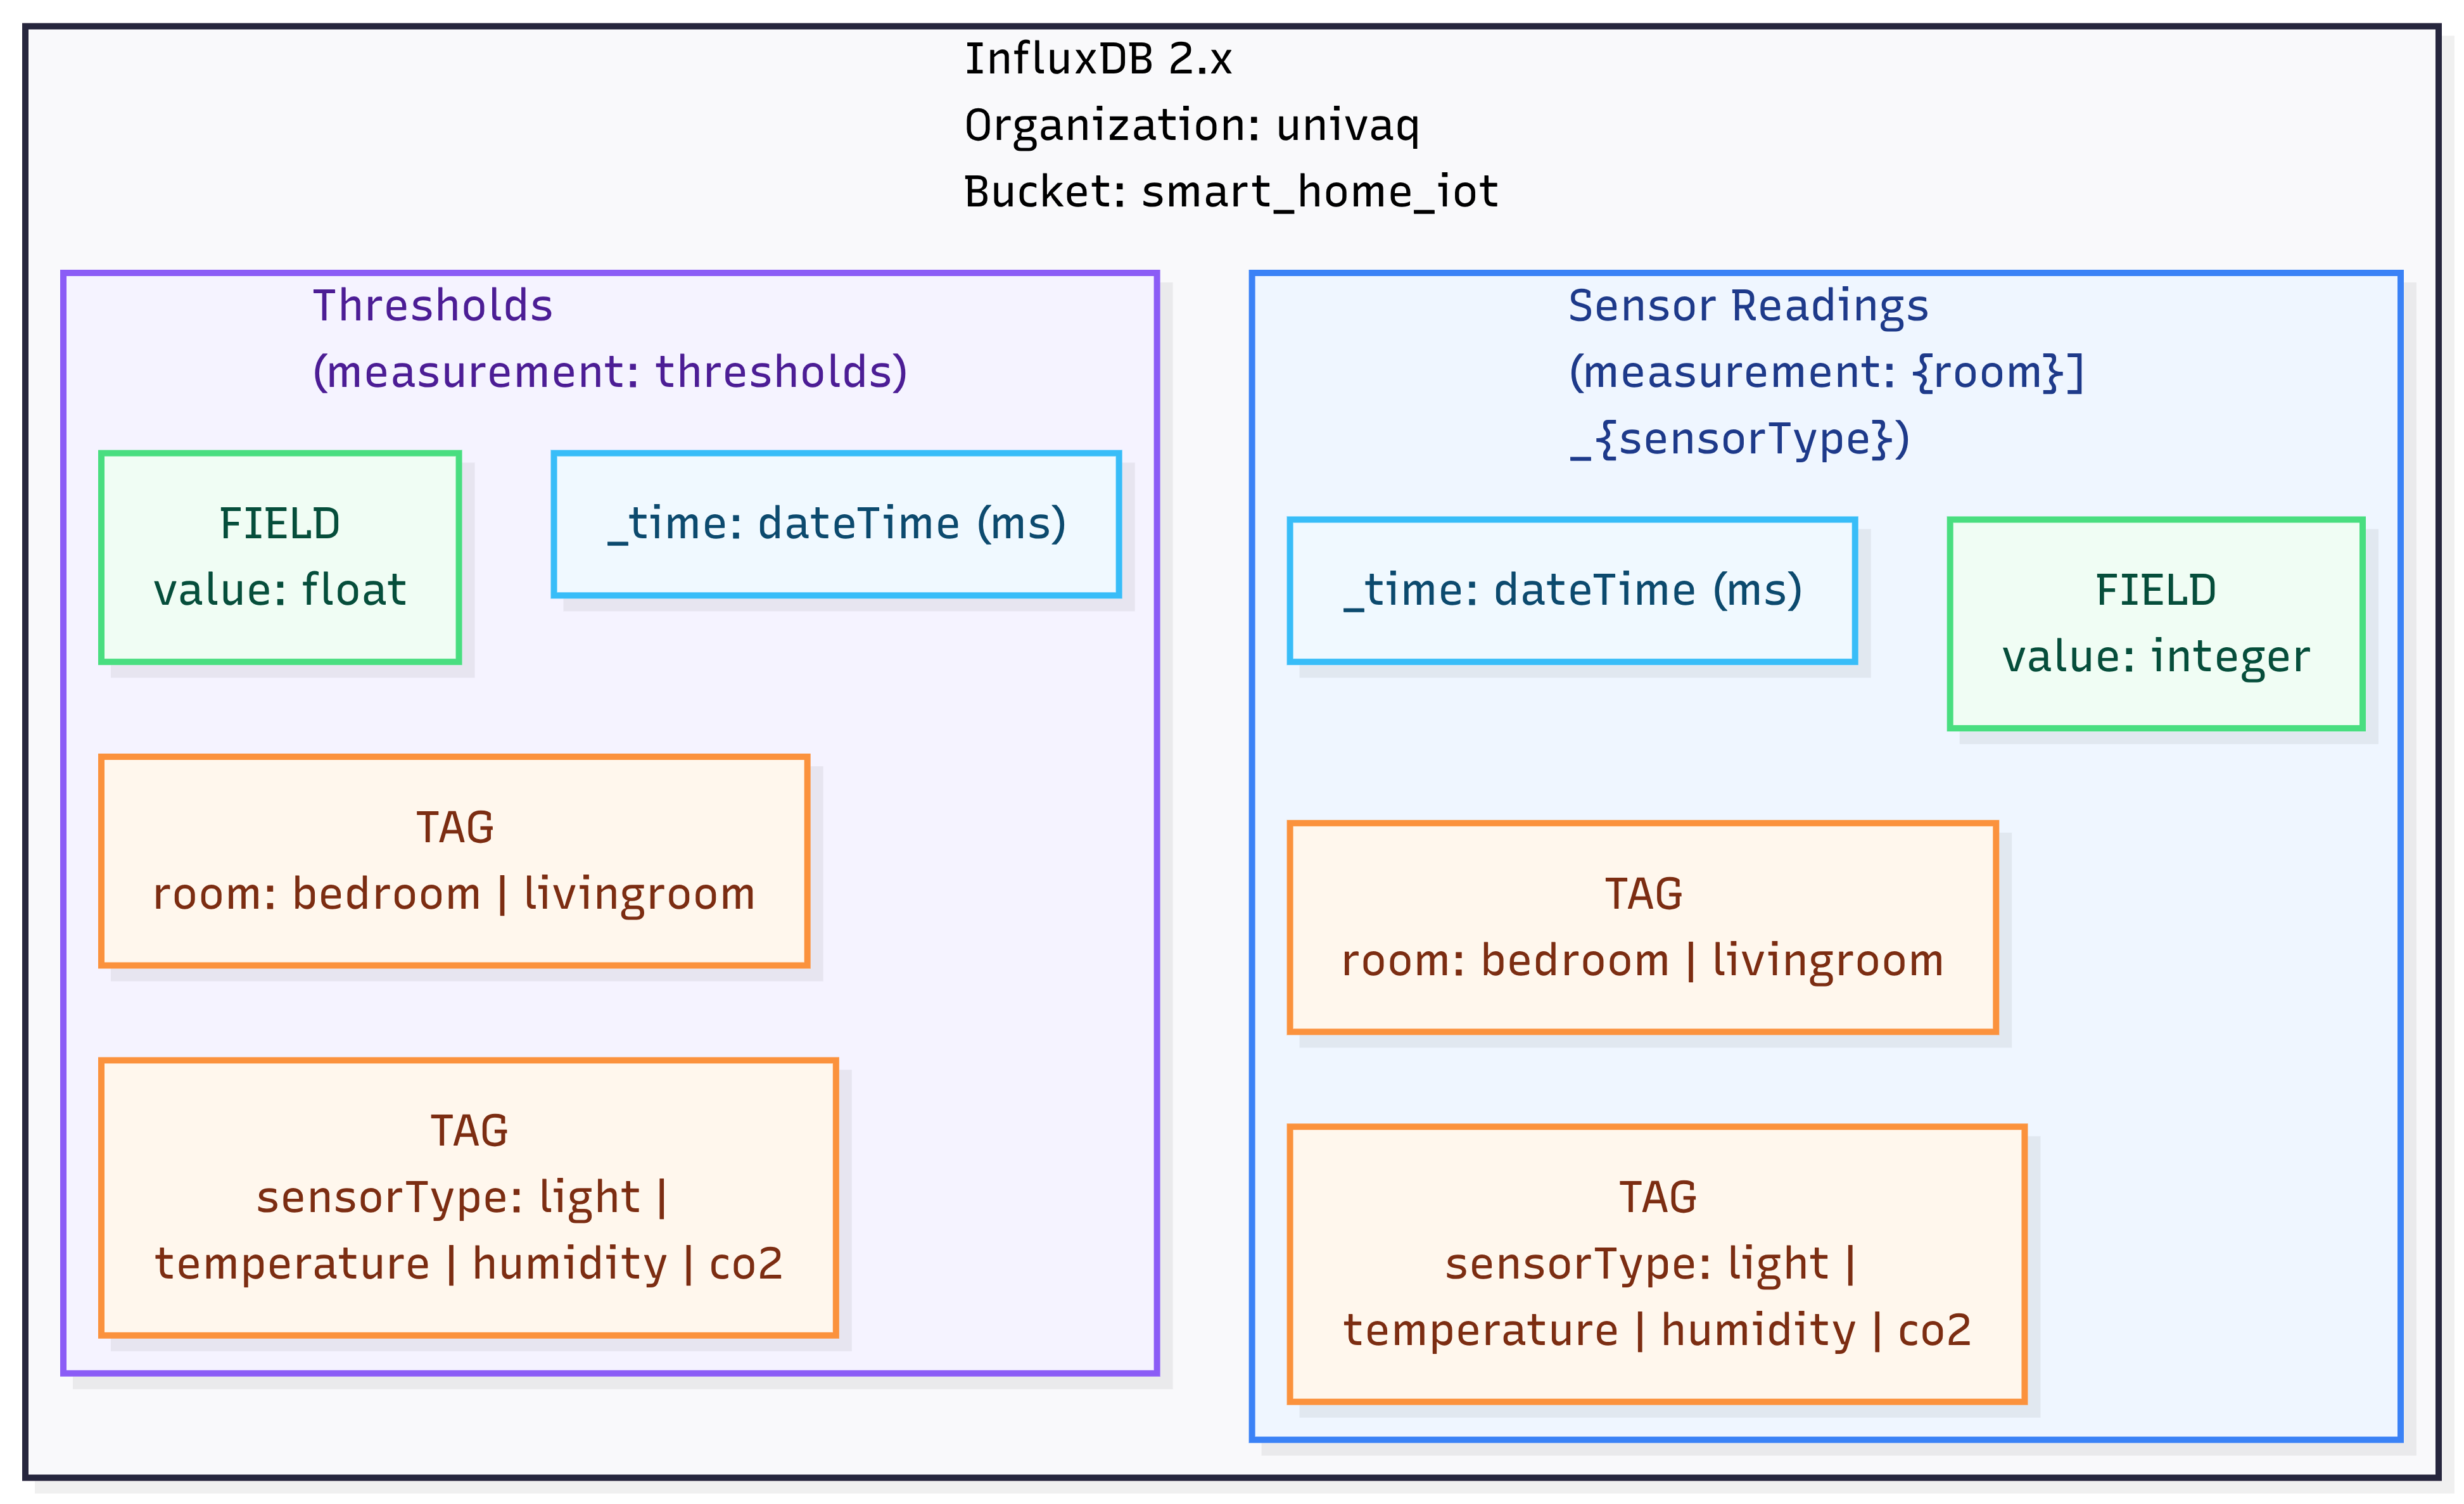
\includegraphics[width=0.8\textwidth]{images/f7database.png}
\caption{InfluxDB data model schema.}
\label{fig:influxdb-schema}
\end{figure}

Sensor readings go into measurements named
\path{{room}_{sensorType}} (e.g., \path{bedroom_light},
\path{livingroom_temperature}). Each point has two tags (\path{room}
and \path{sensorType}) and one integer field (\path{value}) with
millisecond-precision timestamps. Threshold changes are stored in a separate
\path{thresholds} measurement with the same tag structure but a float
\path{value}. Anyone reading the data can reconstruct the full context from
the measurement name and tags alone.

The database initialises automatically at container startup through
\path{DOCKER_INFLUXDB_INIT_*} environment variables that set the admin
credentials, organisation, bucket, and retention policy.

% ---------------------------------------------------------------------------
\section*{5. Visualization}
\addcontentsline{toc}{section}{5. Visualization}
% ---------------------------------------------------------------------------

The requirements ask for an interactive dashboard with real-time graphs,
gauges, filtering, and visual highlighting of threshold violations.

\textbf{Grafana} provisions itself automatically at startup from
configuration files mounted as Docker volumes. A YAML datasource definition
points to InfluxDB with the URL, organisation, bucket, and auth token. A JSON
dashboard definition creates the Smart Home IoT dashboard (uid
\texttt{smarthome-main}).

\begin{figure}[H]
\centering
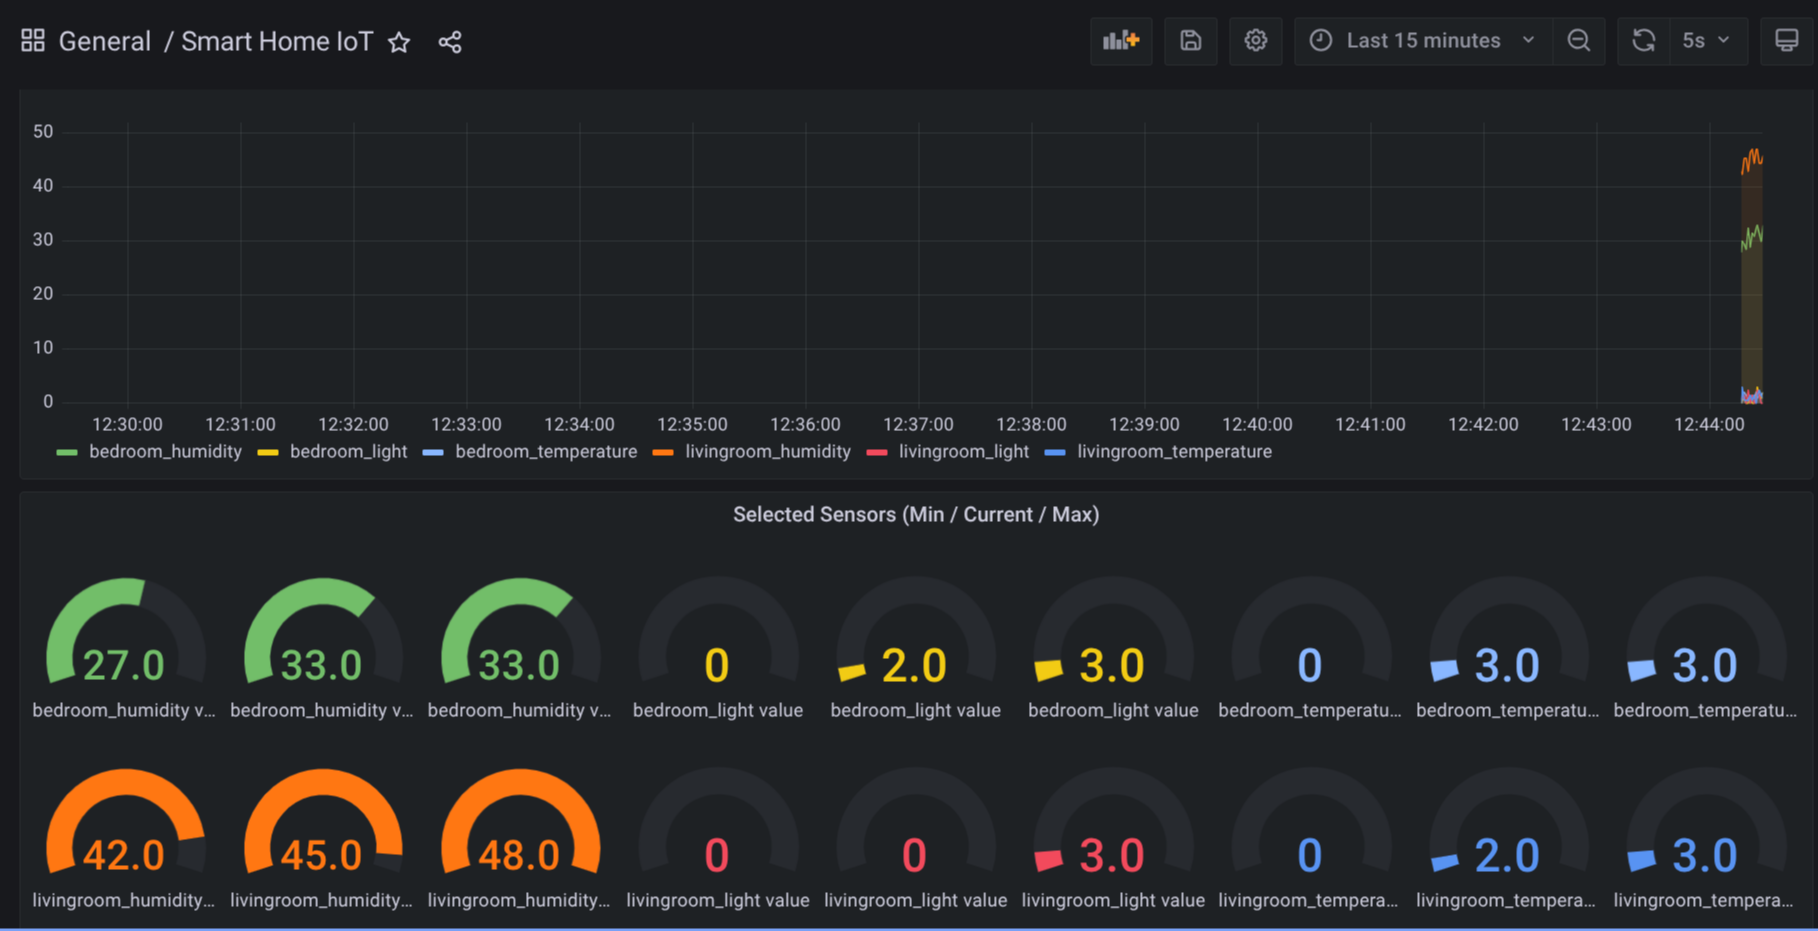
\includegraphics[width=0.9\textwidth]{images/grafana-dashboard.png}
\caption{Grafana dashboard screenshot.}
\label{fig:grafana-dashboard}
\end{figure}

The dashboard has two panels. A time-series line chart shows sensor values
over a configurable time window (default 15 minutes) and refreshes every five
seconds. A gauge panel shows minimum, current, and maximum values for selected
sensors, with threshold violations in red. A template variable
\texttt{\$measurement} lets the user filter by measurement name.

The dashboard uses Flux, the InfluxDB query language. Flux's pipeline syntax
chains filtering, aggregation, and windowing as stream transformations, which
fits the time-series nature of the data.

% ---------------------------------------------------------------------------
\section*{6. Alerting Mechanisms}
\addcontentsline{toc}{section}{6. Alerting Mechanisms}
% ---------------------------------------------------------------------------

The requirements ask for configurable thresholds and notifications through
messaging platforms, with structured messages that identify the domain,
sensor, location, and violated condition.

\textbf{Threshold configuration.} Default thresholds live in the shared file
\path{simulated_env/thresholds.json}. The Manager Application provides a
web interface (port 8089) to view and edit these values at runtime. You can
add new sensors and enable or disable existing ones from the same interface.

\begin{figure}[H]
\centering
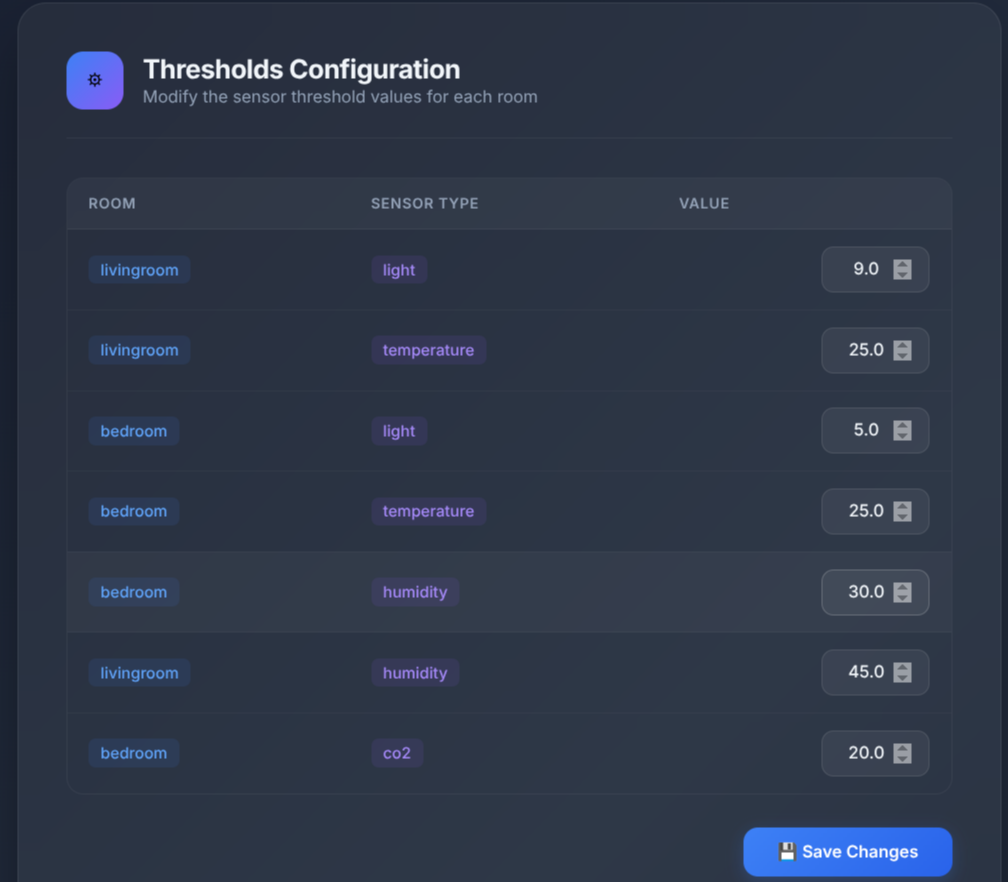
\includegraphics[width=0.8\textwidth]{images/manager-thresholds.png}
\caption{Manager Application threshold management page.}
\label{fig:manager-thresholds}
\end{figure}

\begin{figure}[H]
\centering
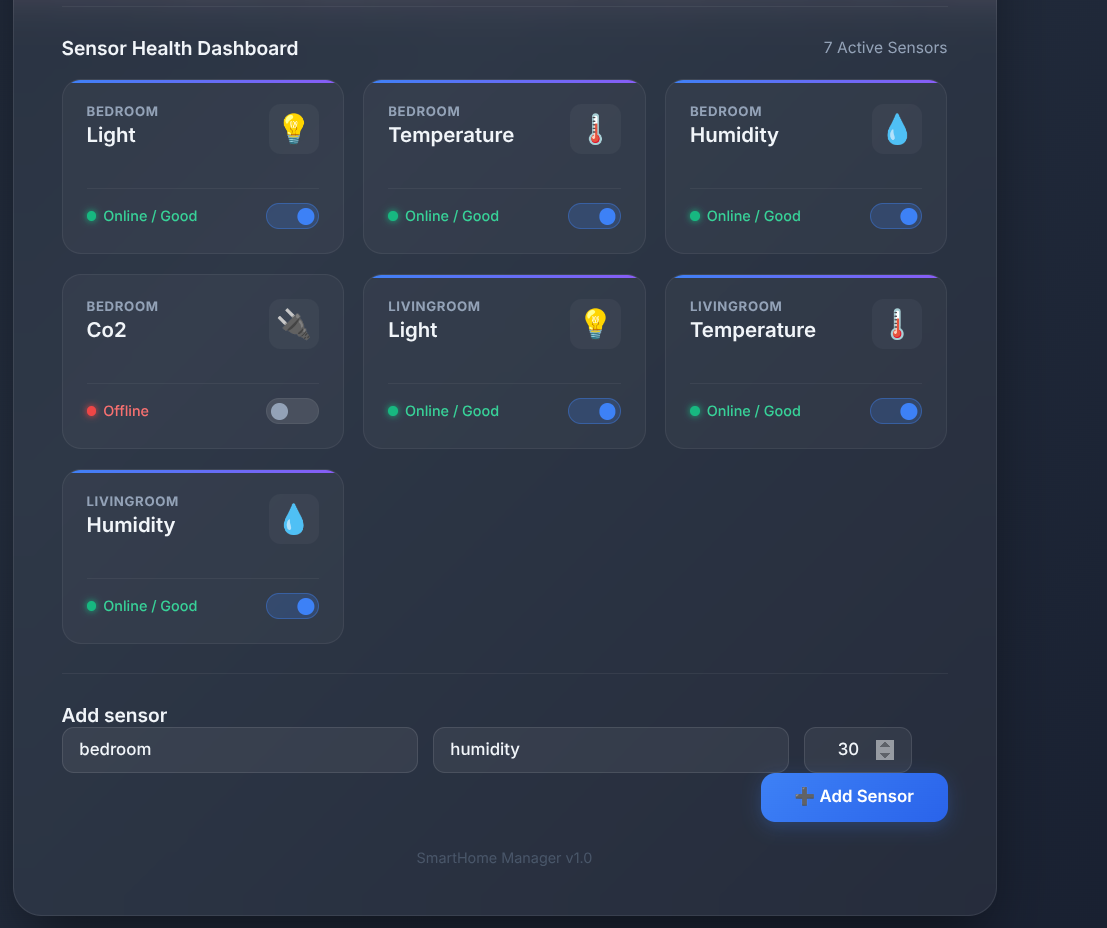
\includegraphics[width=0.8\textwidth]{images/manager-sensors.png}
\caption{Manager Application sensor status and enablement page.}
\label{fig:manager-sensors}
\end{figure}

\textbf{Alert trigger.} Threshold checking happens in Node-RED's threshold
check node. It retrieves the threshold for a sensor from the global context
using the composite key \texttt{\{room\}\_\{sensorType\}}. If the sensor value
exceeds the threshold, the message goes to the alerting sub-flow.

\textbf{Telegram notifications.} The alert sub-flow creates an HTTP POST
request to the Telegram Bot API at
\texttt{https://api.telegram.org/bot<token>/sendMessage}. The message body
uses the structured format from the specification:

\begin{lstlisting}[caption=Alert message format]
Domain: SmartHome
Location: <room>
Sensor: <sensorType>
Condition: Exceeded max value
\end{lstlisting}

The bot token and chat ID come from the environment variables
\texttt{TGBOT\_TOKEN} and \texttt{TG\_CHAT\_ID}.

\textbf{Actuator automation.} When a threshold is breached, the system
notifies and acts. For light sensors it publishes \texttt{"0"} (turn off) to
\texttt{SmartHome/<room>/lightAct}. For temperature sensors it publishes
\texttt{"20"} (set-point) to \texttt{SmartHome/<room>/temperatureAct}. A
debounce limits actuation to one command per five seconds per sensor to avoid
oscillation.

\begin{figure}[H]
\centering
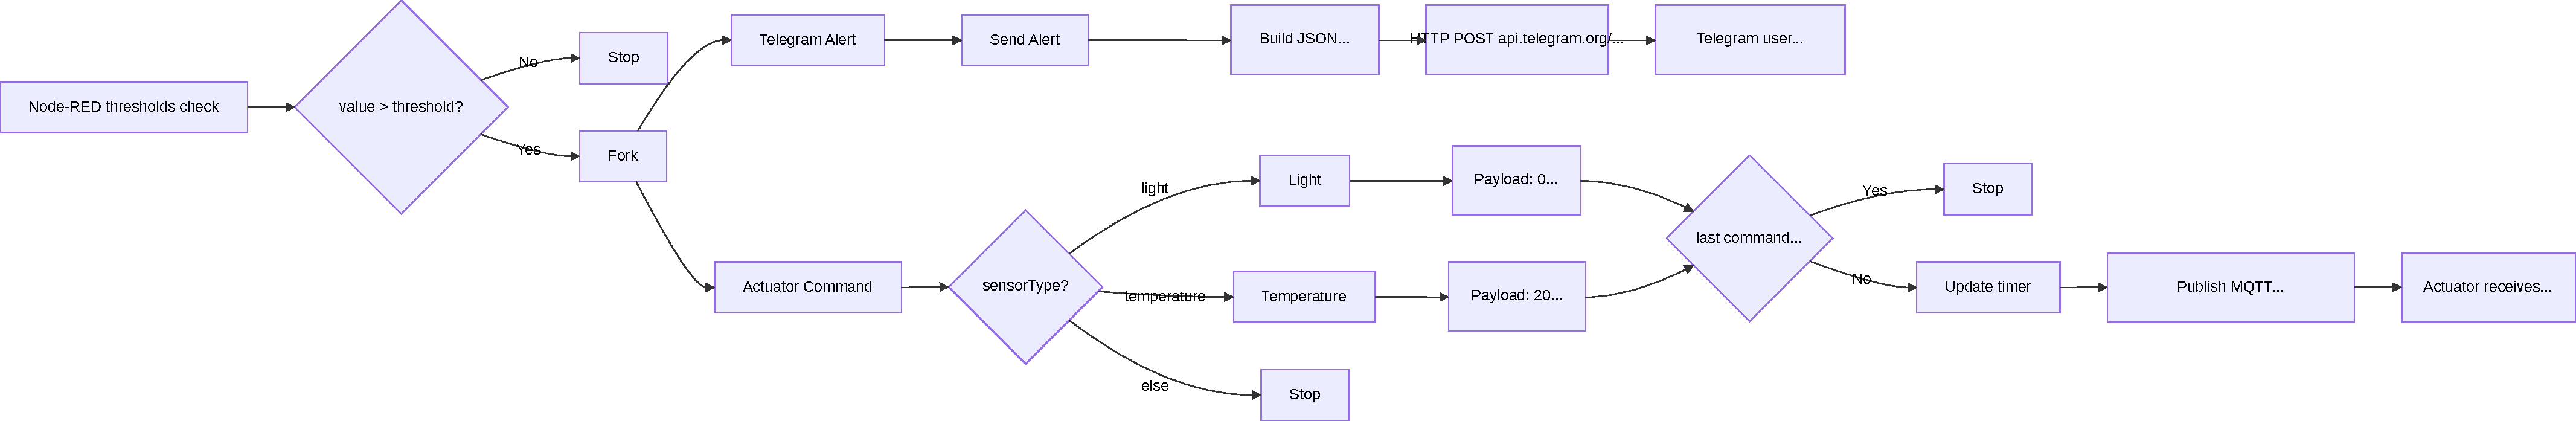
\includegraphics[width=0.8\textwidth]{images/alert-flow.pdf}
\caption{Alert and actuation flow diagram.}
\label{fig:alert-flow}
\end{figure}

% ===========================================================================
\chapter*{Testing}
\addcontentsline{toc}{chapter}{Testing}
% ===========================================================================

Testing an IoT system presents unique challenges. Unlike a standard web
application, an IoT stack spans multiple technologies (MQTT, Node-RED,
InfluxDB, Docker) and failure modes include network interruptions, malformed
messages, file corruption, and misconfigured containers. We structured the
tests into three levels: unit tests for the business logic (Manager
Application), validation scripts for the infrastructure (Docker Compose), and
validation scripts for the processing pipeline (Node-RED flows).

\begin{figure}[H]
\centering
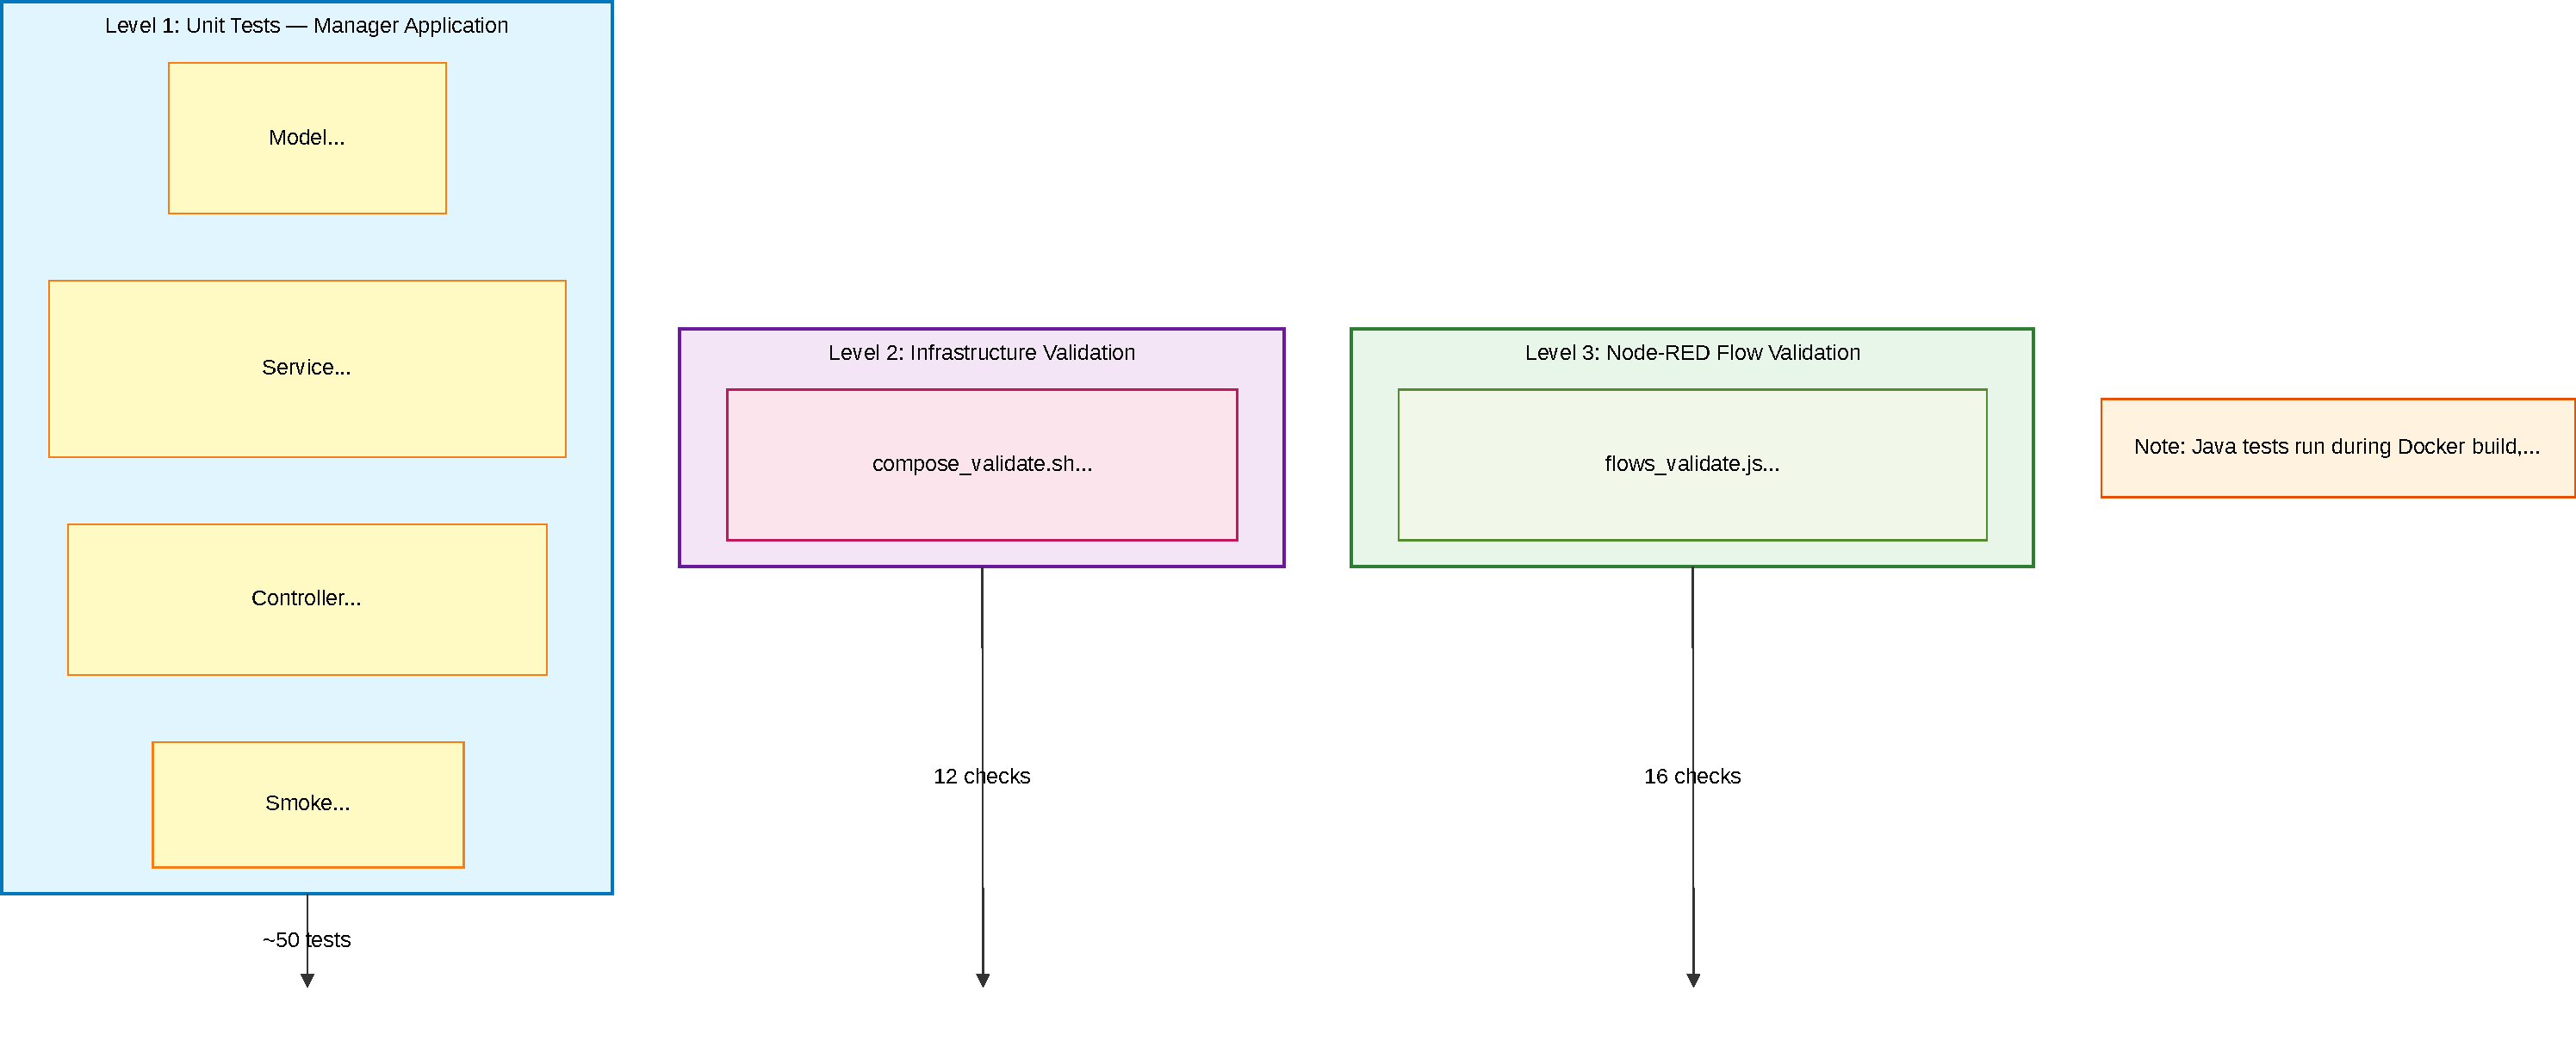
\includegraphics[width=0.8\textwidth]{images/test-levels.pdf}
\caption{Schema of the three test levels and their coverage.}
\label{fig:test-levels}
\end{figure}

\section*{Unit Tests Manager Application}

The Manager Application is the component with the most complex business logic:
it reads and writes JSON files for thresholds and environment state, publishes
MQTT messages, and serves a web UI. We used JUnit 5 with Mockito to test each
layer in isolation.

\subsection*{Model layer}

\textbf{ThresholdTest} verifies that the \texttt{Threshold} POJO correctly
stores room, sensorType, and value. The \texttt{equals()} method is tested
to confirm that two thresholds with the same room and sensorType are
considered equal regardless of their valuea deliberate design choice
since the form submission uses \texttt{equals()} to identify which thresholds
to update.

\textbf{SensorTest} tests the \texttt{Sensor} POJO, including the health
status logic: an enabled sensor has ``Good'' health, while a disabled sensor
is marked ``Offline''. This mapping is used by the web UI to show status
indicators.

\textbf{ThresholdsFormTest} tests the wrapper class used by Thymeleaf to bind
form data. It ensures the form works with an empty list, which can happen
when the thresholds file is missing or empty.

\subsection*{Service layer}

\textbf{ThresholdsServiceImplTest} is the most comprehensive test class. It
uses \texttt{@TempDir} to create isolated JSON files and Mockito to simulate
the MQTT client without requiring a real broker. The tests cover five areas.

GetThresholds validates reading from \texttt{thresholds.json}: a valid file,
an empty array, and a missing file (which should throw IOException).

UpdateThresholds verifies that writing a list of thresholds produces correct
JSON output.

AddThreshold tests the full flow of adding a new sensor: file update,
duplicate detection (IllegalArgumentException for existing room+sensorType),
automatic trimming and lowercasing of names, and synchronisation with
\texttt{env.json}.

GetSensors parses the environment file in both formats the current
structured format (\texttt{\{value, enabled\}}) and the legacy plain integer
format and correctly produces Sensor objects with the right health status.

ToggleSensorStatus verifies enabling and disabling sensors, including the
conversion of legacy plain-integer entries to the structured format when a
sensor is toggled for the first time. Edge cases such as unknown rooms,
unknown sensors, and missing files are handled without throwing exceptions.

PublishThresholdsMQTT tests the scheduled task that broadcasts thresholds
every five seconds. It covers five scenarios: already connected (publishes
directly), disconnected (connects then publishes), multiple thresholds
(publishes to separate topics), connection failure (handles MqttException
gracefully), and missing file (handles IOException gracefully).

\subsection*{Controller layer}

\textbf{ManagerControllerTest} uses \texttt{@WebMvcTest} with MockMvc to test
all four endpoints without starting a full HTTP server. The ten test methods
cover the success path and the error path for each endpoint: GET / returns the
thresholds page, POST /changeThresholds redirects with success or error
messages, POST /addSensor handles success, duplicates, and internal errors,
and POST /sensorEnabled correctly reports the new state (``On'' or ``Off'').

\subsection*{Smoke test}

\textbf{ManagerApplicationTest} is a \texttt{@SpringBootTest} that loads the
full Spring context. If any bean fails to instantiate or a dependency is
missing, the test fails immediately. This catches configuration errors that
unit tests cannot detect.

\begin{figure}[H]
\centering
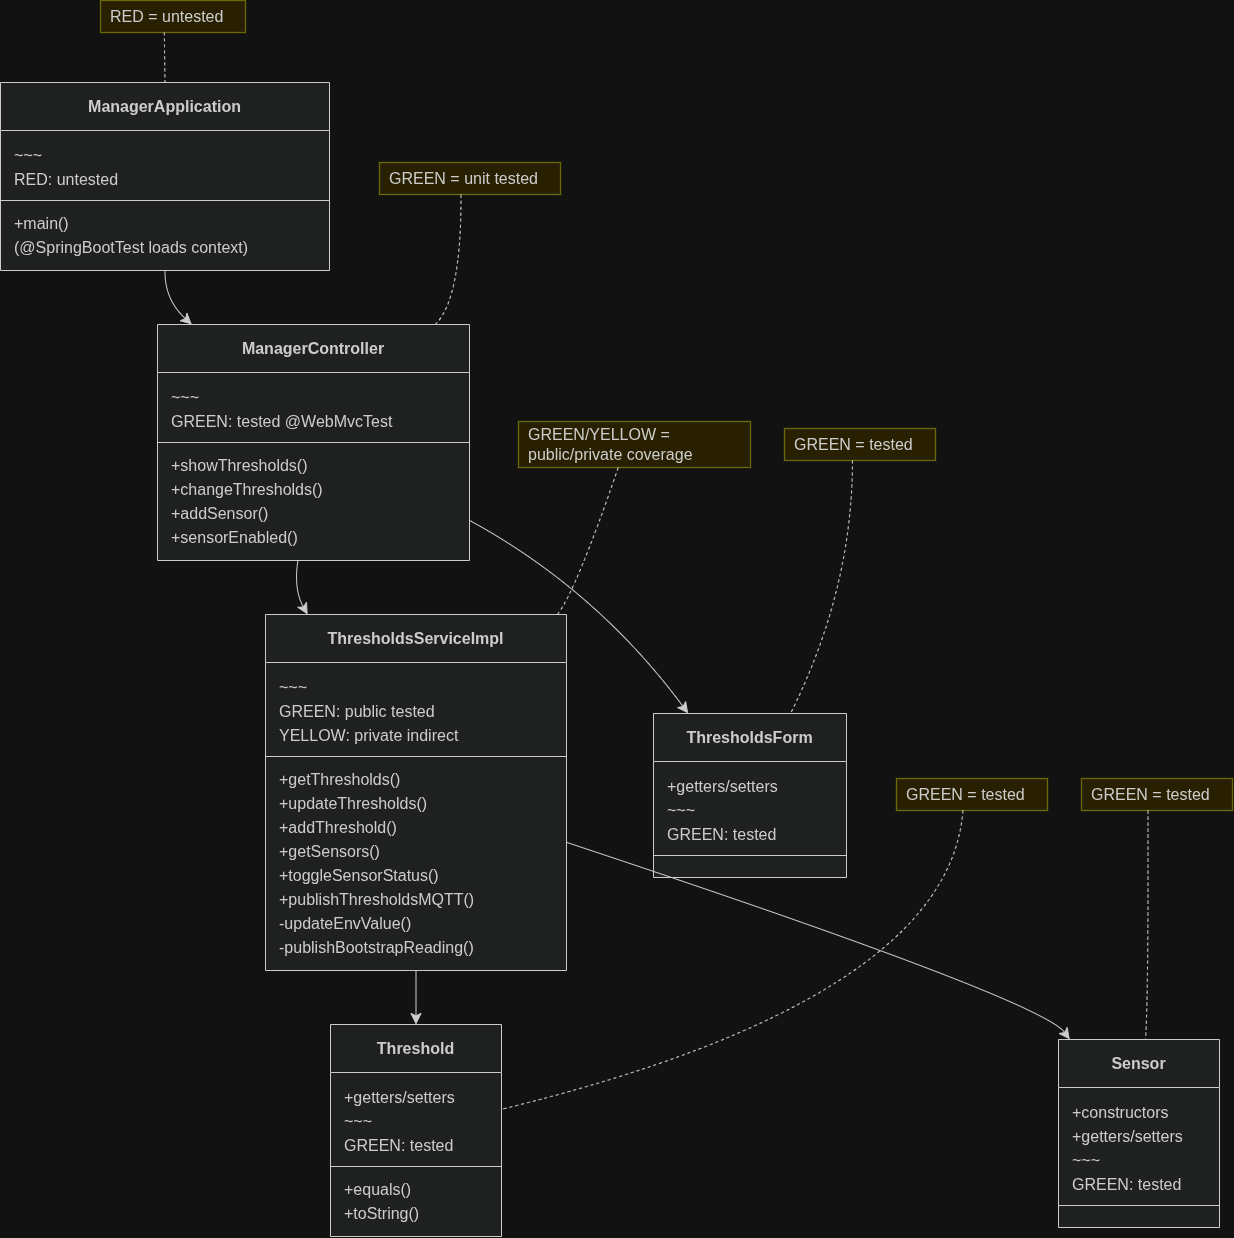
\includegraphics[width=0.8\textwidth]{images/Figure 13_ Manager Application test coverage diagram..drawio.png}
\caption{Manager Application test coverage diagram.}
\label{fig:test-coverage}
\end{figure}

\section*{Infrastructure Validation}

\textbf{compose\_validate.sh} is a bash script that validates the Docker
Compose setup. It checks that \texttt{compose.yaml} is syntactically valid,
the \texttt{.env} file exists, all referenced Dockerfiles and configuration
files are present, every service defines either an image or a build context,
and every service is attached to the \texttt{net-test} network. Since an error
in the compose file blocks the entire deployment, this script acts as a
syntax and sanity gate before running \texttt{docker compose up}.

\section*{Node-RED Flow Validation}

\textbf{flows\_validate.js} validates the Node-RED \texttt{flows.json} file.
The Node-RED flow contains the core processing logic: filtering, parsing,
threshold checking, Telegram alerts, InfluxDB writes, and actuator commands.
An invalid flow causes silent misbehaviour alerts might not fire, data
might not be stored, or actuators might not respond without any error
log. The script checks that the JSON is well-formed, every node has an id and
type, all wire connections point to existing nodes, the JavaScript code in
every Function node is syntactically valid, MQTT nodes reference a configured
broker, and InfluxDB nodes reference a valid configuration.

\section*{How Tests Are Run}

\begin{lstlisting}[caption=Comandi per eseguire i test]
# Unit test della Manager Application
cd managerApplication/app/managerApp && ./mvnw test

# Validazione Docker Compose
./tests/compose_validate.sh

# Validazione Node-RED flows
node tests/flows_validate.js
\end{lstlisting}

The Java tests are also executed automatically during the Docker build, inside
the multi-stage Dockerfile, before the application JAR is packaged. This
prevents a container image from being built if the tests fail.

% ===========================================================================
\chapter*{Non-Functional Requirements}
\addcontentsline{toc}{chapter}{Non-Functional Requirements}
% ===========================================================================

\textbf{Portability.} Every component runs in a Docker container. The whole
stack is defined in one \texttt{compose.yaml} file. All seven containers
connect to a shared bridge network (\texttt{net-test}). Two named volumes
provide persistent storage for InfluxDB and Grafana. The
\texttt{simulated\_env} directory is bind-mounted into the sensors, actuators,
and manager containers for shared file access. One
\texttt{docker compose up -d --build} command deploys everything on any
machine with Docker.

\textbf{Scalability.} The MQTT topic structure separates data streams by room
and sensor type. Adding a new sensor just means publishing to a new topic. No
changes to the broker, Node-RED flows, or database schema are needed. The
Manager Application has an \texttt{addSensor} endpoint to register the new
sensor's threshold and environment entry from the web interface.

\textbf{Resilience.} Actuators retry MQTT connections up to ten times on
connection loss. File operations on the shared environment use exclusive file
locking (\texttt{FileLock}) and atomic renames. Writes go to a temporary file
first, then get atomically moved to the target path. This prevents partial
writes and race conditions when multiple actuators write at the same time.

\textbf{User-Friendly Design.} Grafana auto-provisions on startup with no
manual setup. The Manager Application has a dark-themed web UI with sensor
health indicators, an editable threshold table, and an add-sensor form. The
project README provides quick-start instructions and documentation.

\textbf{Security.} InfluxDB requires authentication through an admin token
configured at startup. Each component exposes only the ports it needs:
Mosquitto on 1883, Node-RED on 1880, InfluxDB on 8086, Grafana on 3000,
Manager App on 8089. The MQTT broker allows anonymous connections in this
development setup. Adding username/password authentication or TLS would be
the first step before moving to production.

\begin{figure}[H]
\centering
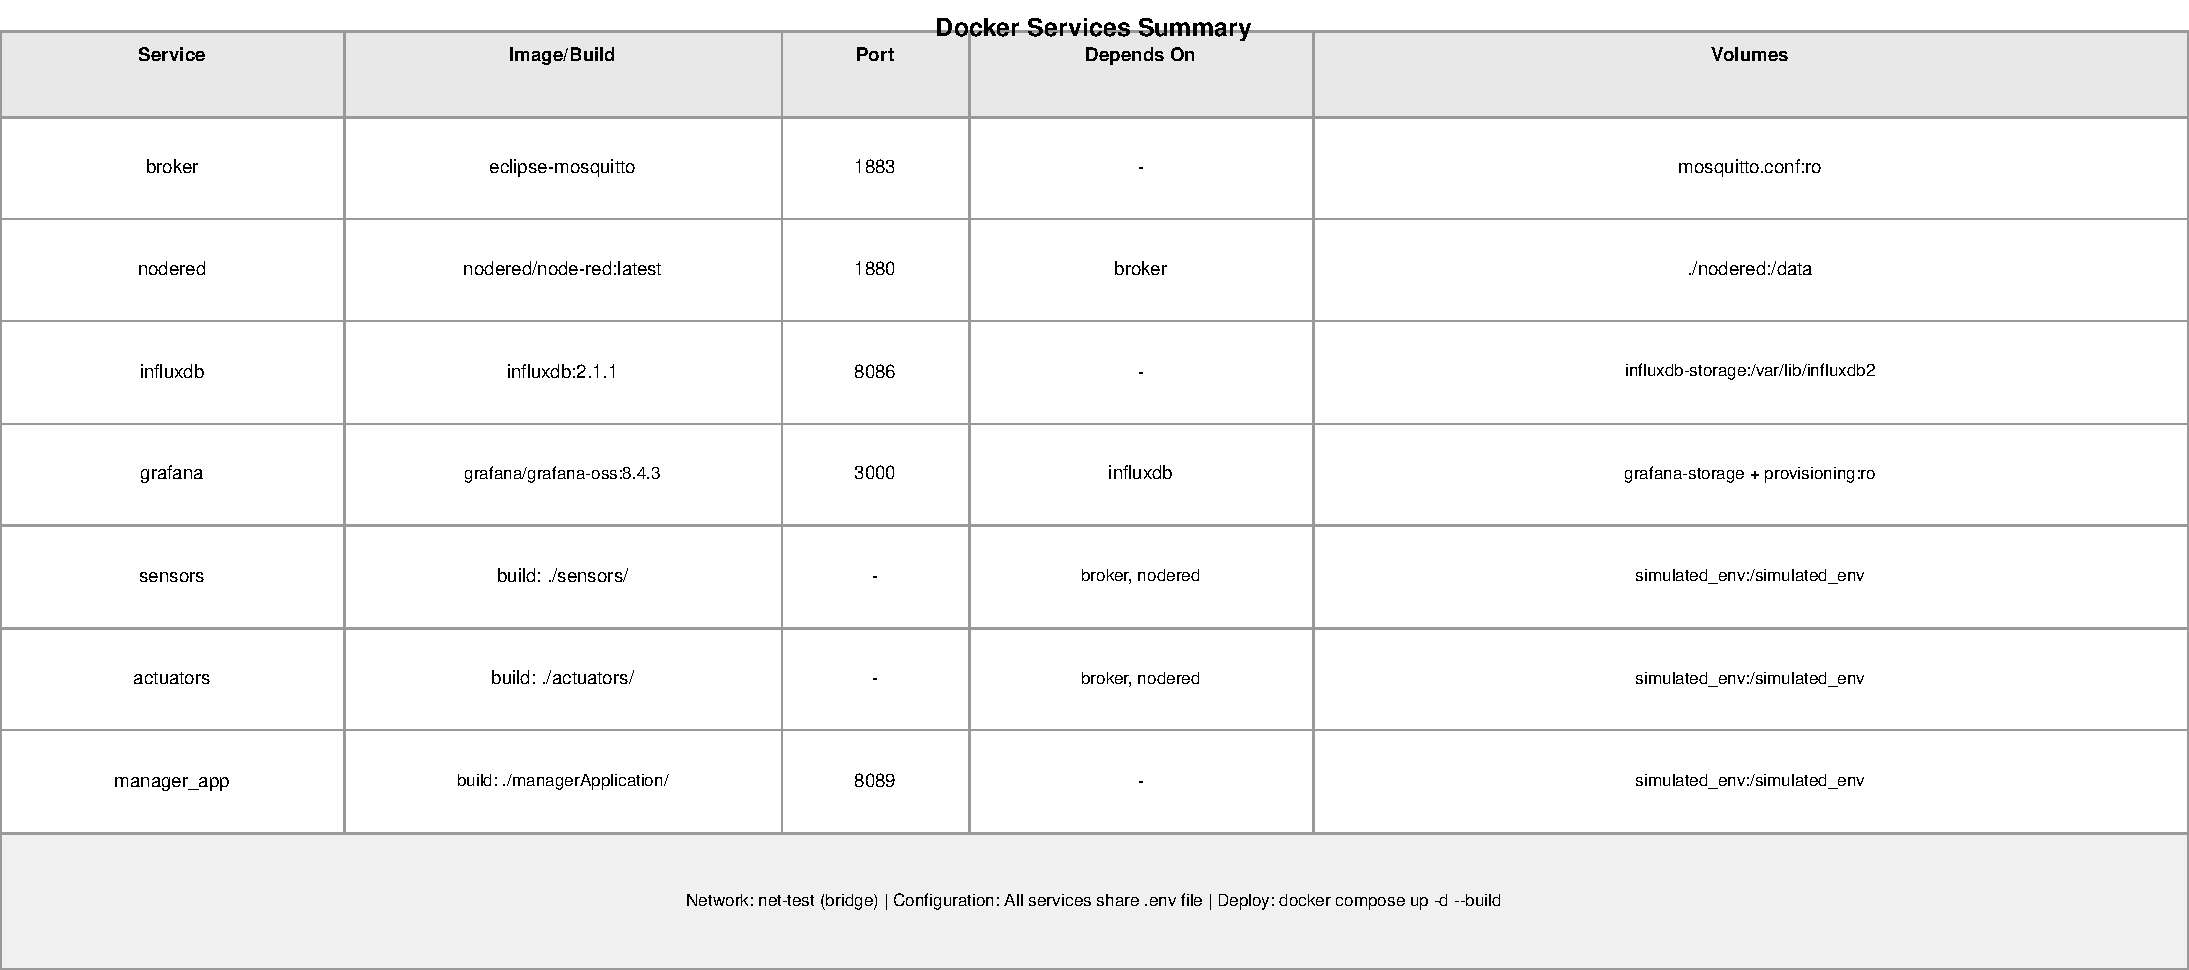
\includegraphics[width=0.8\textwidth]{images/docker-config.pdf}
\caption{Docker configuration summary table.}
\label{fig:docker-config}
\end{figure}

\end{document}
